% Contributors: Jie Li, Yadin Rozov
% Contributors: Kevin Wu, Emily Jin
% Contributors: Jenny Chen, Collin Burns, Nav Ravindranath
% Contributors: Eric Bolton, Xinyuan Cao
\section{Hardness of \emph{k}-means}

In this section, we show that the $k$-means problem is NP-hard. To do
so, we first demonstrate that NAE-3SAT* $\le_p$ Generalized 2-means, and
then that the Generalized 2-means instance constructed in the reduction
of NAE-3SAT* can be solved by 2-means. Since NAE-3SAT* is a decision
problem which is known to be NP-hard, this establishes the NP-hardness
of $k$-means.

To motivate the definition of the Generalized $k$-means problem, we
first reformulate the original $k$-means problem. We initially defined
the $k$-means problem as follows.

\begin{mdframed}
    \underline{\textbf{$k$-means (Formulation 1)}}
    
    \vspace{0.5em} \underline{Input}:
    $\{x_1, \ldots, x_n\} = S \subset \bbR^d$, positive integer $k$
    
    \vspace{0.5em} \underline{Output}: $T \subset \bbR^d$, $|T| = k$
    
    \vspace{0.5em} \underline{Goal}: minimize $\text{cost}(T) :=
    \sum\limits_{s \in S} \min\limits_{t \in T} \norm{s - t}^2$
\end{mdframed}

Equivalently, rather than only outputting a set $T$ of cluster centers,
we could instead output a partition of the input set $S$. This gives a
second formulation of $k$-means.

\begin{mdframed}
    \underline{\textbf{$k$-means (Formulation 2)}}
    
    \vspace{0.5em} \underline{Input}:
    $\{x_1,\ldots,x_n\} = S \subset \bbR^d$, positive integer $k$
    
    \vspace{0.5em} \underline{Output}: $P_1, \ldots, P_k \subset [n],
    ~\bigcup_{j=1}^k P_j = [n],
    ~P_j \cap P_{j'} = \emptyset ~\text{for}~ j \ne j';$

    $\quad \mu_1, \ldots, \mu_k \in \bbR^d,
    ~\mu_j ~\text{is the center of the points in cluster}~ P_j$
    
    \vspace{0.5em} \underline{Goal}: minimize
    $\text{cost}(P_1, \ldots, P_k, \mu_1, \ldots, \mu_k) :=
    \sum\limits_{j=1}^k \sum\limits_{i \in P_j} \norm{x_i - \mu_j}^2$
\end{mdframed}

Finally, we make use of the following fact to remove the necessity to
explicitly know the cluster centers.

\begin{fact}
    $\E \norm{X - \E X}^2 = \frac{1}{2} \E_{X,Y} \norm{X - Y}^2
    \quad (X, Y ~\text{i.i.d.})$
\end{fact}

\begin{proof}
    \begin{align*}
        \E_{X,Y} \norm{X - Y}^2
        &= \E_{X,Y} \left[(X - Y)^2\right] \\
        &= \E_X \E_Y \left[X^2 + Y^2 - 2 X Y\right] \\
        &= \E X^2 + \E Y^2 - 2 \E_X \E_Y [X Y] \\
        &= 2 \left[\E X^2 - (\E X)^2\right] \\
        &= 2 \E \left[(X - \E X)^2\right] \\
        &= 2 \E \norm{X - \E X}^2
    \end{align*}
\end{proof}

Observing that each cluster center $\mu_j := \frac{1}{|P_j|}
\sum_{i \in P_j} x_i$ can be thought of as an expectation of the points
in belonging to $P_j$, and applying the previous fact, we see that
\begin{align*}
    \sum_{j=1}^{k} \sum_{i \in P_j} \norm{x_i - \mu_j}^2
    &= \sum_{j=1}^{k} \sum_{i \in P_j} \norm{x_i - \frac{1}{|P_j|}
        \sum_{i' \in P_j} x_{i'}}^2 \\
    &= \sum_{j=1}^{k} \frac{1}{2 |P_j|} \sum_{i,i' \in P_j}
        \norm{x_i - x_{i'}}^2
\end{align*}
which leads to yet another formulation of $k$-means.

\begin{mdframed}
    \underline{\textbf{$k$-means (Formulation 3)}}
    
    \vspace{0.5em} \underline{Input}:
    $\{x_1,\ldots,x_n\} = S \subset \bbR^d$, positive integer $k$
    
    \vspace{0.5em} \underline{Output}: $P_1, \ldots, P_k \subset [n],
    ~\bigcup_{j=1}^k P_j = [n],
    ~P_j \cap P_{j'} = \emptyset ~\text{for}~ j \ne j'$
    
    \vspace{0.5em} \underline{Goal}: minimize
    $\text{cost}(P_1, \ldots, P_k) := \sum\limits_{j=1}^{k}
    \frac{1}{2 |P_j|} \sum\limits_{i,i' \in P_j} \norm{x_i - x_{i'}}^2$
\end{mdframed}

A slight modification of this last formulation leads to the Generalized
$k$-means problem; instead of using the squared distance penalty term
$\norm{x_i - x_{i'}}^2$, we can specify the penalties as an $n \times n$
matrix $D$ with the entry $D_{ii'}$ giving the penalty for points $x_i$
and $x_{i'}$.

\begin{mdframed}
    \underline{\textbf{Generalized $k$-means}}
    
    \vspace{0.5em} \underline{Input}:
    $n \times n$ symmetric matrix $D$, positive integer $k$
    
    \vspace{0.5em} \underline{Output}: $P_1, \ldots, P_k \subset [n],
    ~\bigcup_{j=1}^k P_j = [n],
    ~P_j \cap P_{j'} = \emptyset ~\text{for}~ j \ne j'$
    
    \vspace{0.5em} \underline{Goal}: minimize
    $\text{cost}(P_1, \ldots, P_k) := \sum\limits_{j=1}^{k}
    \frac{1}{2 |P_j|} \sum\limits_{i,i' \in P_j} D_{ii'}$
\end{mdframed}

\subsection{Review of NP-hard problems}
\begin{enumerate}
\item Problems that are NP-hard admit polynomial time
  reductions from all other problems in NP.
\item To carry out such a necessary reduction that proves a problem is NP-hard, the following steps can used (\cite{cor2009}): 
\begin{enumerate}
\item Given an instance $\alpha$ of a problem $A$ that has previously
  been proven to be NP-hard ($A \in NP$), use a polynomial time algorithm to transform it to an instance $\beta$ of problem $B$ .
\item Run a decision algorithm for $B$ on instance $\beta$ 
\item Use the answer for $\beta$ to get $\alpha$
\end{enumerate} 
\end{enumerate} 

For a more complete review of complexity and hardness please go to
reference \cite{cor2009} chapter 34.

Our goal is to show that the 2-means problem is NP hard:

\begin{theorem}\label{2-means-np-hard}
2-means clustering is an NP-hard optimization problem
\end{theorem} 

Approach to the problem is based on \cite{das2008}.  To prove this we
will start with the known NP-hard problem of 3SAT and show a reduction
from it to the NAE-3SAT* problem.  From that problem we will show a
reduction to the Generalized 2-means problem and finally show a
reduction from that to the 2-means problem. \\

In each reduction  we need to show how an instance of the known NP-hard problem can be modified in polynomial time into an instance of the problem we want
to show is NP-hard, and vice versa. In other words, we must show that the reduction maps a 'yes'
instance of the known problem to a 'yes' instance of the new problem
and 'no' instance of the known problem to a 'no' instance of the new
problem. Note since the set NP is a set of \emph{decision problems}, the
input of an instance of a problem must include the decision threshold
for the problem.

We'll briefly review NP-completeness, only to the extent necessary to
set the stage for this proof.  A more thorough treatment can found in
a computational complexity course. As a consequence of the Cook-Levin
Theorem, which pointed to the first NP-hard problem, we know that SAT
and variations, such as 3SAT and NAE 3-SAT, are NP-hard.

\subsection{Hardness proof preliminaries}
\begin{definition}[3SAT]
\item \underline{Input}:  A 3-CNF Boolean formula over $n$ literals. 
\begin{itemize}
\item 3-CNF (3-Conjunctive Normal Form): A Boolean formula that can be expressed as an \emph{AND} over
  $m$ clauses, each of which is an \emph{OR} over exactly 3 literals.
\end{itemize}
\item \underline{Output}: \emph{True} if there exists, \emph{False} if not.
\end{definition}

\begin{definition}[NAE 3-SAT] \emph{NAE 3-SAT} or
  \emph{not-all-equal-3SAT} is a 3SAT formula, with the additional
  requirement that, in each clause at least one literal is true and at
  least one literal is false.  This removes the case where all three
  literals in a clause are true.   
\end{definition}

\begin{definition}[NAE 3-SAT*] 
A boolean formula $\phi$ containing $n$ literals $x_1,...x_n$.
Exactly 3 literals for each of $m$ clauses.  Each pair of variables
$x_i$, $x_j$ appears in at most 2 clauses.  Once as $(x_i,x_j)$ or
$(\neg x_i, \neg x_j)$ and once as  $(x_i,\neg x_j)$ or $(\neg x_i,
x_j)$. 
\end{definition}

\begin{definition}[Generalized 2-means]
\item \underline{Input}: $n \times n$ matrix, ``distance matrix'' with
    elements $D_{ii'} =$ distance between object $i$ and object $i'$
\item \underline{Output}: Partition of objects into $P_1$ and $P_2$
\item \underline{Goal}: minimize $cost(P_1,P_2) := \sum\limits_{j=1}^{2}
    \frac{1}{2|P_j|} \sum\limits_{i,i' \in P_j} D_{ii'}$. 
\end{definition}


\begin{lemma}[Hardness of NAE-3SAT*] \label{np-nae-3-sat}
See \cite{das2008}. (??)
\end{lemma}

\subsection{Hardness of generalized 2-means}

For any instance $\phi$ of $x_1,...x_n$ of NAE-3SAT* we construct a
$2n \times 2n$ distance matrix $D_{\alpha,\beta}$ as below where
$\alpha,\beta \in x_1,...x_n, \neg x_1,....,\neg x_n$.  Note that
because the definition of NAE-3SAT* requires that each pair of
variables $x_i$, $x_j$ appears in at most 2 clauses, once as
$(x_i,x_j)$ or $(\neg x_i, \neg x_j)$ and once as  $(x_i,\neg x_j)$ or
$(\neg x_i, x_j)$ , the matrix is uniquely defined for a given
$\phi$. 
\begin{definition}[Distance matrix for generalized
    2-means] \label{2-means-distance-matrix} Define
  $D(\phi)$ by:
\begin{align}
  D_{\alpha,\beta} = \begin{cases}
    0 & \textrm{if } \alpha = \beta\\
    1+\Delta  & \mbox{if } \alpha = \overline{\beta} \\
    1+\delta  & \mbox{if } \alpha \sim \beta \\
    1 & \textrm{otherwise}.
  \end{cases}
\end{align}
Where $ \alpha \sim \beta$ means that either $\alpha$ and $\beta$
occur together in a clause or $\alpha$ and $\overline{\beta} $ occur
together in a clause, where:
\begin{align}
  \Delta = \frac{5m}{5m + 2n} \quad\textrm{and}
  \quad\delta = \frac{1}{5m  + 2n}.
\end{align}
\end{definition}
Note that above implies that $0 < \delta < \Delta < 1$ and also:
\begin{align}
4 \delta m < \Delta \le 1 - 2 \delta n.
\end{align}

Consider the following example matrix generated from the clause $x_1 \vee \bar{x_2} \vee x_3$, where the diagonal is filled with 0s (where $\alpha=\beta$).

\begin{table}[H]
\begin{tabular}{lllllll}
                       & $x_1$                      & $x_2 $                     & $x_3 $                    & $\bar{x_1}$                      & $\bar{x_2}$                      & $\bar{x_3}$                     \\ \cline{2-7} 
\multicolumn{1}{l|}{$x_1$} & \multicolumn{1}{l|}{0} & \multicolumn{1}{l|}{1}  & \multicolumn{1}{l|}{1+$\delta$}  & \multicolumn{1}{l|}{1+$\Delta$}  & \multicolumn{1}{l|}{$1+\delta$}  & \multicolumn{1}{l|}{1}  \\ \cline{2-7} 
\multicolumn{1}{l|}{$x_2$} & \multicolumn{1}{l|}{1}  & \multicolumn{1}{l|}{0} & \multicolumn{1}{l|}{1}  & \multicolumn{1}{l|}{1+$\delta$}  & \multicolumn{1}{l|}{1+$\Delta$}  & \multicolumn{1}{l|}{1+$\delta$}  \\ \cline{2-7} 
\multicolumn{1}{l|}{$x_3$} & \multicolumn{1}{l|}{1+$\delta$}  & \multicolumn{1}{l|}{1}  & \multicolumn{1}{l|}{0} & \multicolumn{1}{l|}{1}  & \multicolumn{1}{l|}{1+$\delta$}  & \multicolumn{1}{l|}{1+$\Delta$}  \\ \cline{2-7} 
\multicolumn{1}{l|}{$\bar{x_1}$} & \multicolumn{1}{l|}{1+$\Delta$}  & \multicolumn{1}{l|}{1+$\delta$}  & \multicolumn{1}{l|}{1}  & \multicolumn{1}{l|}{0} & \multicolumn{1}{l|}{1}  & \multicolumn{1}{l|}{1+$\delta$}  \\ \cline{2-7} 
\multicolumn{1}{l|}{$\bar{x_2}$} & \multicolumn{1}{l|}{1+$\delta$}  & \multicolumn{1}{l|}{1+$\Delta$}  & \multicolumn{1}{l|}{1+$\delta$}  & \multicolumn{1}{l|}{1}  & \multicolumn{1}{l|}{0} & \multicolumn{1}{l|}{1}  \\ \cline{2-7} 
\multicolumn{1}{l|}{$\bar{x_3}$} & \multicolumn{1}{l|}{1}  & \multicolumn{1}{l|}{1+$\delta$}  & \multicolumn{1}{l|}{1+$\Delta$}  & \multicolumn{1}{l|}{1+$\delta$}  & \multicolumn{1}{l|}{1}  & \multicolumn{1}{l|}{0} \\ \cline{2-7} 

\end{tabular}

\end {table}

We want to reformulate Generalized k-means from a minimization problem to a decision problem to prove satisfiability, so we prove the following lemma.
\begin{lemma} \label{generalized-2-means-cost}
$\phi$ is NAE-3SAT* satisfiable if and only if $D(\phi)$ admits a
generalized 2-means cost of $cost(\phi) = n - 1 + \frac{2\delta
  m}{n}$. 
\end{lemma}

\begin{proof}
Partition the corresponding matrix object ($2n$ object) for the
NAE-3SAT* satisfied $\phi$ into two partitions; one for all the
literals that are assigned \textit{true} and a second for all literals
that are assigned \textit{false}.  Since each literal is represented
twice we have $|P_1| = |P_2| = n$.   By definition of the NAE-3SAT*,
each clause contributes one pair to $P_1$ and pair to $P_2$.   Also
this leads to the fact that the distances between pairs can only be 1,
$1+\delta$, with $m$ instances of the later and the fact that the two
clusters have identical costs. So we get that 
\begin{align*}
cost(P_1,P_2) &= \sum_{j=1}^{2} \frac{1}{2|P_j|} \sum_{i,i' \in P_j}
D_{ii'}\\ 
&= \frac{1}{2n}( 2 {n \choose 2} + 2m\delta ) + \frac{1}{2n}( 2 {n
  \choose 2} + 2m\delta ) \\ 
&= \frac{ n (n-1) } {n} + \frac{2 m \delta}{n} \\
&= n - 1 +  \frac{2 m \delta}{n}
\end{align*}
\end{proof}

\begin{lemma} \label{different-partitions}
For any partition $P_1$ and $P_2$, WLOG $P_1$ contains a variable and
its negation, with $cost(P_1,P_2) \ge n - 1 + \frac{\Delta}{2n} > n -
1 + \frac{2m\delta}{n} = cost(\phi).$ 
\end{lemma}

\begin{proof}
Let $n' = |P_1|$.  Note
\begin{align*}
cost(P_1,P_2) &\ge \frac{1}{n'}({n' \choose 2} + \Delta ) +
\frac{1}{2n-n'}{2n-n' \choose 2}  \\ 
&= n - 1 + \frac{\Delta}{n'} \ge n-1 +\frac{\Delta}{2n}.
\end{align*}
\end{proof}

\begin{figure}
    \centering
    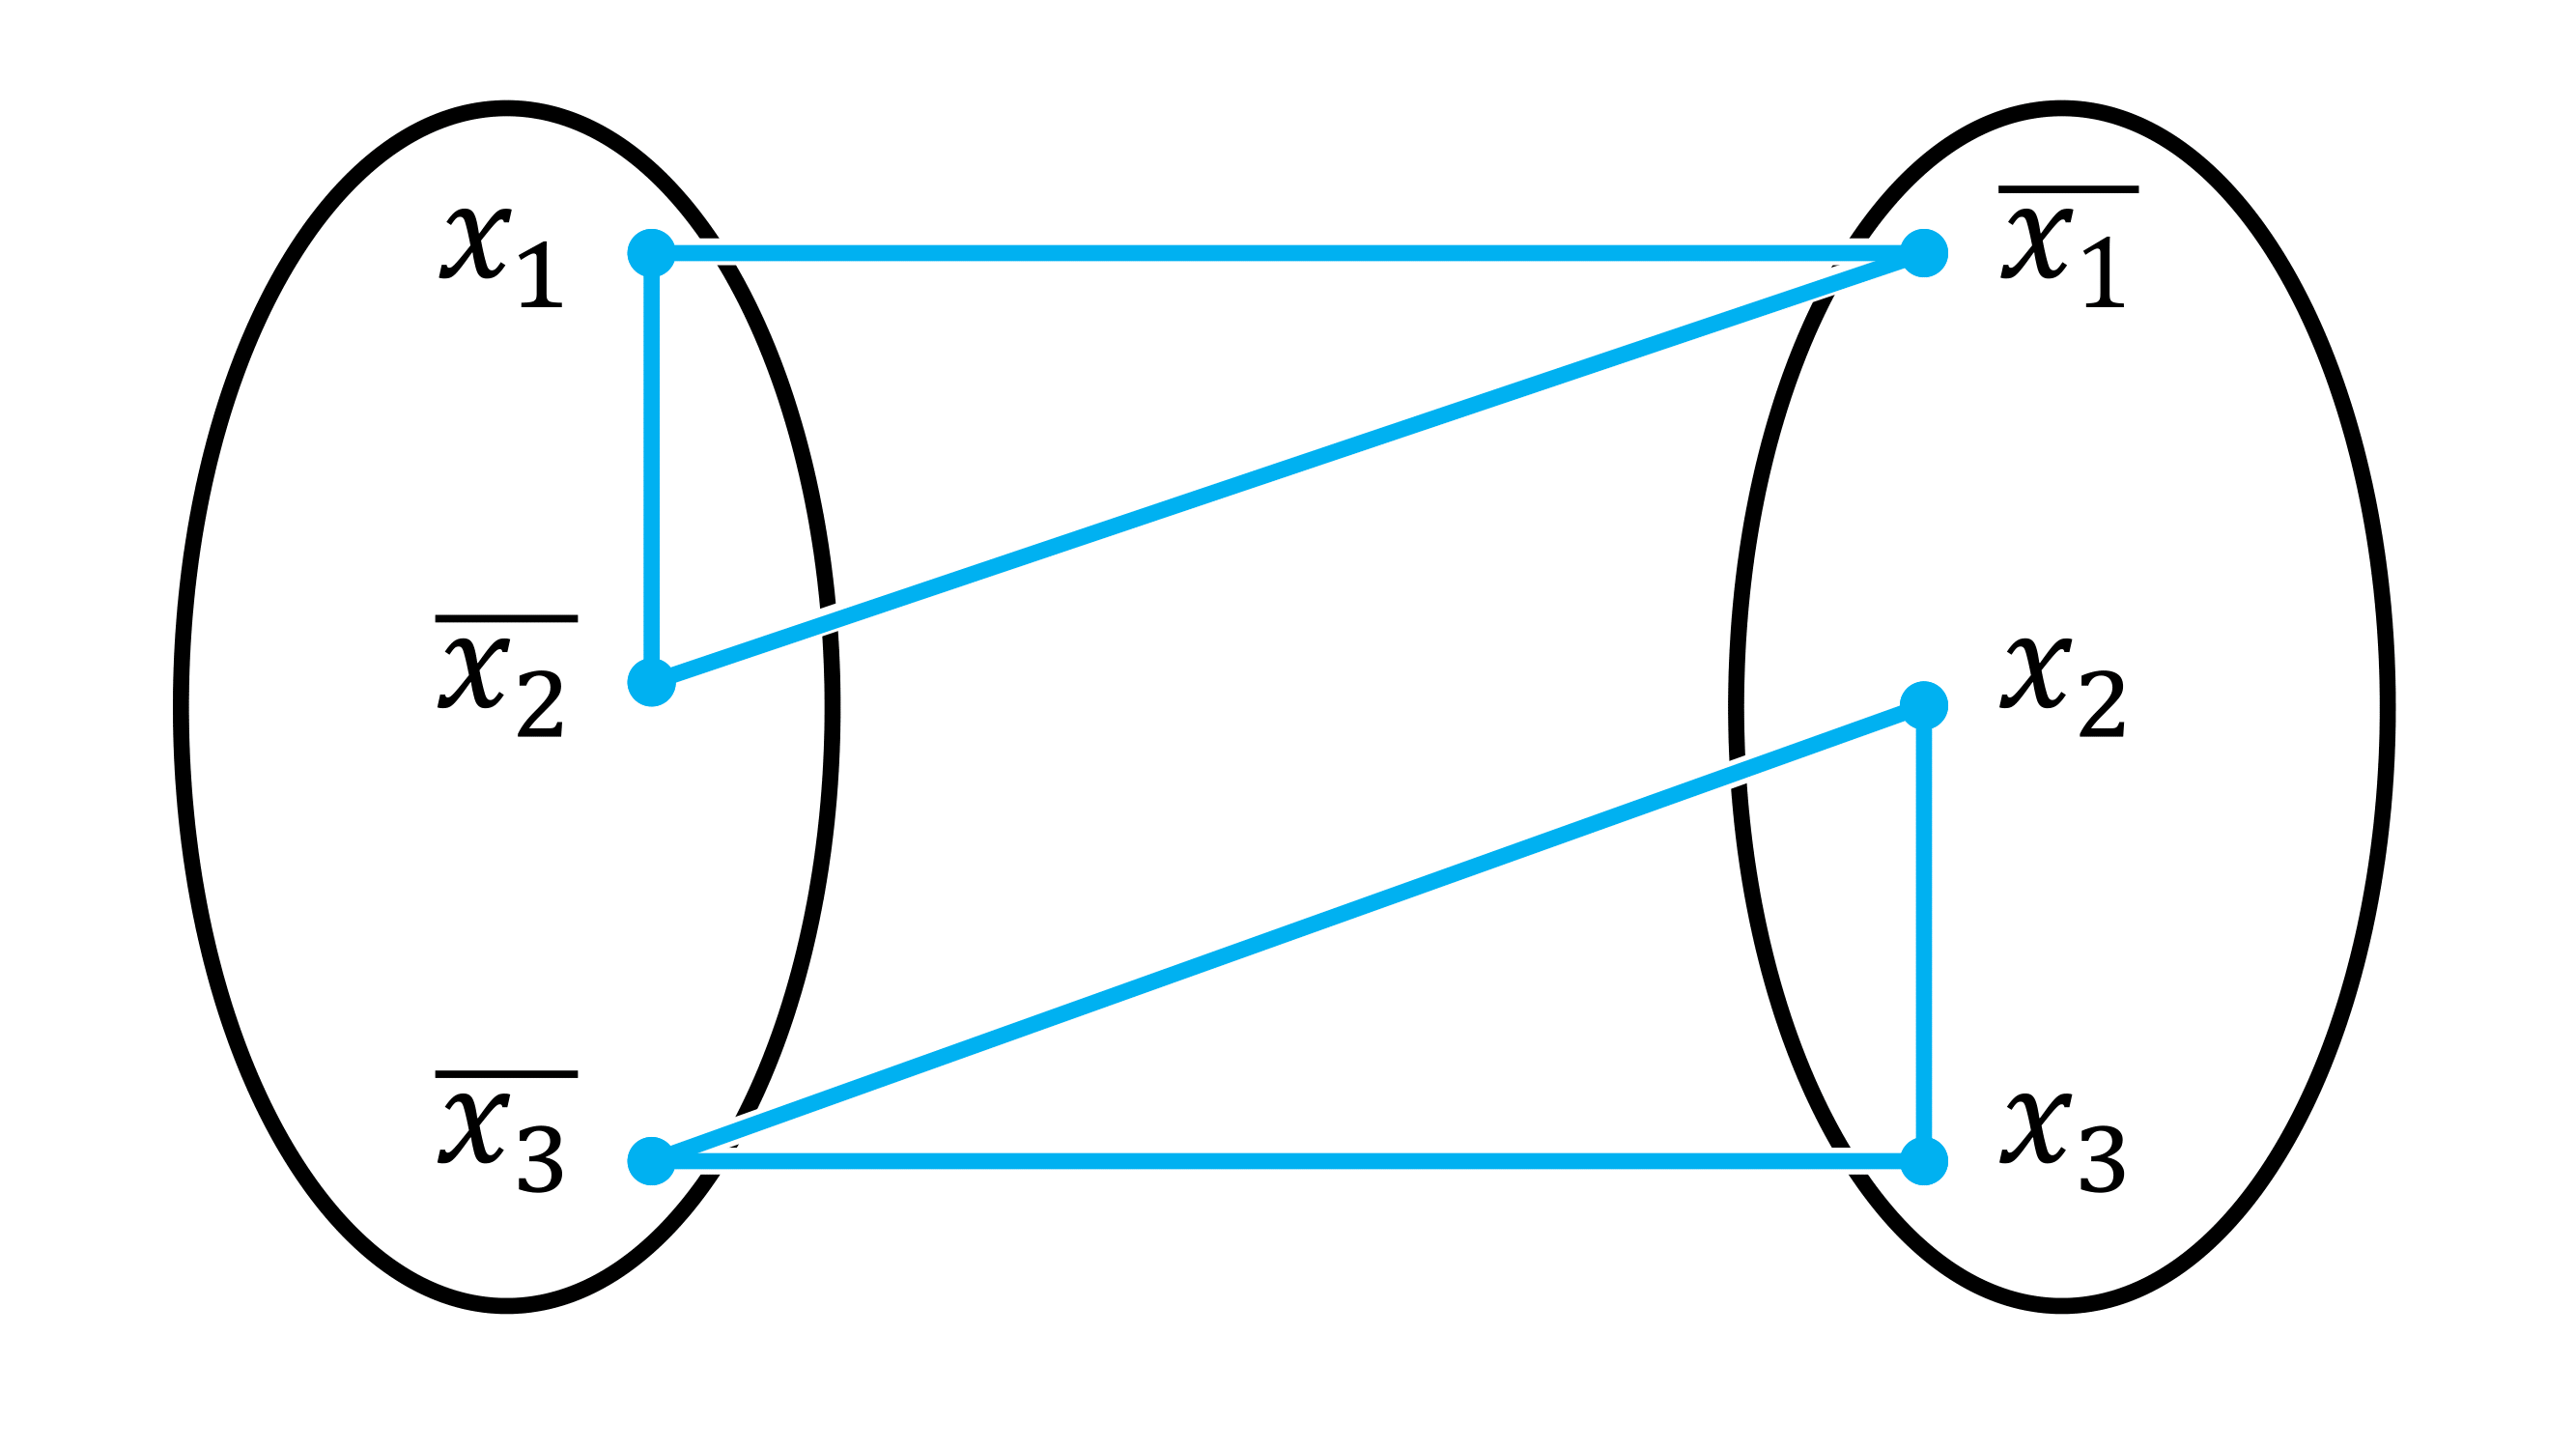
\includegraphics[width=10cm]{chapter_1/files/KmeansNAE3SAT.png}
\centering
    \caption{Partition of True and False literals, with blue lines meaning a cost of $1+\delta$, demonstrating that each clause contributes only $1+\delta$ cost within its cluster.}
    \label{fig:my_label}
\end{figure}


\begin{lemma} \label{satisfiable-instance}
If $D(\phi)$  admits a generalized 2-means cost of $cost(\phi) \le n -
1 + \frac{2\delta m}{n}$, then $\phi$ is a satisfiable instance of
NAE-3SAT*. 
\end{lemma}

\begin{proof}
Let $P_1$ and $P_2$ be the partition with cost $\le n - 1 +
\frac{2\delta m}{n}$.  First note that $P_1$ and $P_2$ do not contain
a variable and its negation and $|P_1| = |P_2| = n$.  The cost of
clustering $P_1$ and $P_2$ is:
\begin{align*}
  \frac{2}{n} \left[ {n \choose 2} + \delta \sum_{\textrm{clauses}} 
  \begin{cases}
    1 & \textrm{if clause is split across $P_1$ and $P_2$}\\  
    3 & \textrm{otherwise} \\ 
  \end{cases}\right]
\end{align*}
Since $cost(P_1, P_2) \le n - 1 + \frac{2\delta m}{n}$, it follows that all
clauses are split between $P_1$ and $P_2$.  That is, every clause has
at least one literal in $P_1$ and one literal in $P_2$.  Therefore,
the assignment that sets all of the $P_1$ to true and all of $P_2$ to
false is a valid NAE-3SAT* assignment. 
\end{proof}



\subsection{Generalized 2-means to 2-means}
We will use the hardness of generalized 2-means to show the hardness
of 2-means by embedding $D(\phi)$.
\begin{fact}
Note that any $n \times n$ symmetric matrix $D$ can be embedded in
$l_2^2$ iff $u^TDu  \le 0$ for all $u \in \mathbb{R}^n$ s.t. $\sum u_i
= 0$. 
\end{fact}
\begin{proof}[Proof as homework exercise]
\end{proof}

\begin{fact} \label{d-phi-fact}
For $D(\phi)$, the following holds:
\begin{align*}
u^TDu &= \sum_{\alpha, \beta} u_\alpha u_\beta D_{\alpha \beta}\\ 
&=\sum_{\alpha, \beta} u_\alpha u_\beta (1 - \mathbf{1}_{(\alpha =
  \beta)} + \Delta\mathbf{1}_{(\alpha = \bar{\beta})} + \delta
\mathbf{1}_{(\alpha \sim \beta)})\\ 
&=\sum_{\alpha, \beta} u_\alpha u_\beta - \sum_{\alpha} u_\alpha^2
+2\Delta (u^+ \cdot u^-) + \delta \sum_{\alpha, \beta} u_\alpha
u_\beta \mathbf{1}_{(\alpha \sim \beta)}\\ 
& \le (\sum u_\alpha)^2  - \norm{u}^2 + 2\Delta (u^+ \cdot u^-) +
\delta \sum_{\alpha, \beta} |u_\alpha| |u_\beta| \textrm{,  and use: }
  2ab \le a^2 + b^2\\  
& \le - \norm{u}^2 + \Delta (\norm{u^+}^2  + \norm{u^-}^2) + \delta
(\sum |u_\alpha|)^2 \\ 
& \le -(1- \Delta) \norm{u}^2  + \delta 2n \norm{u}^2 \textrm{,  and
    since } (1- \Delta) \ge \delta 2n \\ 
& \le 0.
\end{align*}
\end{fact}


\begin{proof}[Proof of Theorem~\ref{2-means-np-hard}]
NAE-3SAT* is NP hard from Lemma~\ref{np-nae-3-sat}.  From
Definition~\ref{2-means-distance-matrix} and
Lemmas~\ref{generalized-2-means-cost}, \ref{different-partitions},
\ref{satisfiable-instance} we have that any instance of the NAE-3SAT*,
$\phi$ of $x_1,...x_n$ can be reduced to an instance of the (decision
version of the) generalized 2-means problem with $D(\phi)$ and
threshold $cost(\phi)$.  We also have from the Lemma that with these
specific instances that NAE-3SAT* is solved, \textbf{if and only if}
the generalized 2-means problem is solved.  This combined with the
fact that the reduction steps take polynomial time in $n$ and
Fact~\ref{d-phi-fact} that $D(\phi)$ can be embedded into $l_2$,
completes the proof for 2-means. 
\end{proof}
